\documentclass[a4paper]{report}

\usepackage[T1]{fontenc} % codifica dei font per l'italiano
\usepackage[utf8]{inputenc} % lettere accentate da tastiera
\usepackage[italian]{babel} % lingua del documento
\usepackage[shortlabels]{enumitem}%per fare elenchi ad hoc
\usepackage{framed}% per riquadrare il testo
\usepackage[big]{layaureo} %per avere i margini più stretti
\usepackage{graphicx} %per inserire le immagini

\graphicspath{ {./images/} }

\begin{document}

\chapter*{Economia}
\section*{Bilancio}

\subsection*{Logiche:}

\begin{itemize}
    \item Di Competenza $\longrightarrow$ Segno l'entrata/uscita quando mi accordo che esca/entri (es. emissione scontrino)
    \item Di Cassa $\longrightarrow$ Segno solo quando esce/entra effettivamente (es. scambio di soldi per prodotto)
\end{itemize}

\subsection*{Struttura}
\begin{itemize}
    %====
    \item Stato Patrimoniale (stato dell'azienda) \begin{itemize}
        \item Attivo (cosa ho) \begin{itemize}
            \item Corrente (AC)
            \item Non Corrente (ANC)
            \item Capitale Investito (CI)
        \end{itemize}
        \item Passivo (a chi lo devo) \begin{itemize}
            \item Patrimonio Netto (PN)
            \item Corrente (Debiti) (PC)
            \item Non Corrente (Debiti) (PNC)
            \item Capitale Investito (CI)
        \end{itemize}
    \end{itemize}
    %====
    \item Conto Economico (flussi economici, secondo logica di Competenza)\begin{itemize}
        \item Ricavi dalle Vendite (R)
        \item MON= Ricavi - Costi Operativi
        \item Utile Lordo in funzionamento (UL) = MON - Oneri e Proventi Finanziari (F)
        \item Utile Netto in funzionamento (UN)= UL - Imposte
        \item Utile Netto d'esercizio (UE) = UN - Straordinari
    \end{itemize}
    \item Rendiconto Finanziario (la cassa, secondo logica di Cassa) \begin{itemize}
        \item CF Operativo (CFO)
        \item Cf Investimento
        \item Cf Finanziamento
    \end{itemize}
\end{itemize}

\subsection*{Indici}
\begin{itemize}
    \item Analisi di redditività: \begin{itemize}
        \item ROE = $\frac{UE}{PN}$ (\%)
        indica la remunerazione percentuale del capitale proprio
        \item ROI = $\frac{MON}{CI}$ (\%)
        indicatore della redditività della gestione operativa
        \item ROS = $\frac{MON}{R}$ (\%)
        indica la capacità dell’azienda di produrre risultato operativo dalle
        vendite
        \item ROT = $\frac{R}{CI}$
        ricavo netto medio generato da ogni unità di capitale
        investito nell'attività dell'azienda
        \item r = $\frac{F}{D}$ (\%)
        indica il costo medio del
        capitale di terzi
        \item s = $\frac{UE}{UL}$ saldo della gestione fiscale e delle discontinued operations
        \item $\frac{D}{PN}$ o $\frac{D}{E}$ o rapporto di leva
    \end{itemize}
    Tra l'altro:
    \[
    ROE=[ROI+\frac{MT}{E}(ROI-r)]*s     
    \]
    \item Analisi di Liquidità  \begin{itemize}
        \item Af = $\frac{PN}{CI}$ autonomia finanziaria
        \item Ef = $\frac{PC}{CI}$  elasticità ai finanziamenti
    \end{itemize}
    \item Analisi di Solidità Patrimoniale \begin{itemize}
        \item RC = $\frac{AC}{PC}$ Rapporto Corrente, se >1.5 eccesso Liquidità
        \item EqML = $\frac{CFO}{PNC}$  Equilibrio di Medio-Lungo periodo, l'inverso ci da gli anni cassa necessari a ripagare i Debiti
    \end{itemize}
\end{itemize}

\section*{Investimento}
\[
NCF=CF-I-(\Delta Imp )   
\]
\begin{figure}[h]
    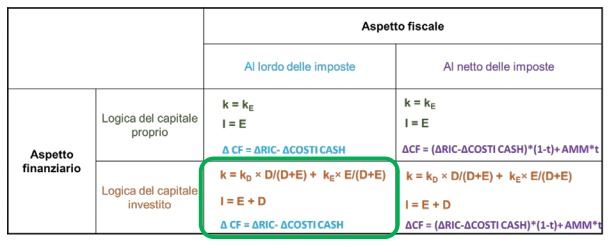
\includegraphics[width=\textwidth]{SchemaInv.jpeg}
    \end{figure}
Se sono al netto delle imposte e ho un k al lordo lo moltiplico per $(1-t)$
\begin{center}
    $\Delta$ Imp =  $\Delta$ Utile * t = ($\Delta$ R - $\Delta$ C - $\Delta$ AMM)
\end{center}
\textbf{Attenzione:} Se l'Utile di uno dei due casi è minore o uguale di 0 devo calcolare "a mano" il $\Delta$ Imposte
e devo tenere in conto anche i Costi Affondati.
\[
V_T = V_m - (V_m-V_b)*t    
\]
\end{document}
